\section*{Výsledky měření}
Teplota v místnosti byla \SI{25.6}{\degreeCelsius}.
Atmosférický tlak byl \SI{992}{\hecto\pascal}.
Relativní vlhkost vzduchu byla \SI{33}{\percent}.
Hustota vzduchu $\sigma$ je při těchto podmínkách přibližně \SI{1.18(1)}{\kg\per\m\cubed}.


V rotačním viskozimetru jsme měřili glycerin a škrob.
Teplota obou kapalin byla \SI{25.6}{\degreeCelsius}.
V kuličkovém pouze glycerin při teplotách v rozmezí \SI{25}{\degreeCelsius} až \SI{35}{\degreeCelsius}.

Naměřené hodnoty viskozity glycerinu jsou uvedeny v tabulce \ref{tab::glyc} zaneseny do grafu \ref{grp::rotglyc}.
Viskozita glycerinu na frekvenci otáčení nijak zřejmě nezávisí (Pearsonův korelační koeficient \num{0.04}).
Glycerin proto považujeme za newtonovskou kapalinu.
Viskozitu určíme metodou nejmenších čtverců, $\eta = $\SI{720(30)}{\milli\Pa\s}.

\begin{tabulka}[htbp]
\centering
\begin{tabular}{ccc|ccc}
rotor & frekvence (\si{\per\minute}) & viskozita (\si{\milli\pascal\s}) & rotor & frekvence (\si{\per\minute}) & viskozita (\si{\milli\pascal\s}) \\
\hline 
\multirow{9}{*}{L1} & \num{0.6} & 861 & \multirow{6}{*}{L2} & 5 & 828 \\
& 1 & 801 & & 6 & 792 \\
& 1.5 & 754 & & 10 & 644 \\
& 2 & 721 & & 12 & 605 \\
& 2.5 & 657 & & 20 & 610 \\
& 3 & 653 & & 30 & 590 \\
& 4 & 667 & & &  \\
& 5 & 661 & \multirow{5}{*}{L3} & 20 & 940 \\
& 6 & 656 & & 30 & 760 \\
&   &     & & 50 & 760 \\
\multirow{2}{*}{L4} & 100 & 740 & & 60 & 740 \\
& 200 & 720 & & 100 & 750 \\
\end{tabular}
\caption{Naměřená viskozita glycerinu rotačním viskozimetrem}
\label{tab::glyc}
\end{tabulka}


\begin{graph}[htbp] 
\centering
% GNUPLOT: LaTeX picture with Postscript
\begingroup
  \makeatletter
  \providecommand\color[2][]{%
    \GenericError{(gnuplot) \space\space\space\@spaces}{%
      Package color not loaded in conjunction with
      terminal option `colourtext'%
    }{See the gnuplot documentation for explanation.%
    }{Either use 'blacktext' in gnuplot or load the package
      color.sty in LaTeX.}%
    \renewcommand\color[2][]{}%
  }%
  \providecommand\includegraphics[2][]{%
    \GenericError{(gnuplot) \space\space\space\@spaces}{%
      Package graphicx or graphics not loaded%
    }{See the gnuplot documentation for explanation.%
    }{The gnuplot epslatex terminal needs graphicx.sty or graphics.sty.}%
    \renewcommand\includegraphics[2][]{}%
  }%
  \providecommand\rotatebox[2]{#2}%
  \@ifundefined{ifGPcolor}{%
    \newif\ifGPcolor
    \GPcolorfalse
  }{}%
  \@ifundefined{ifGPblacktext}{%
    \newif\ifGPblacktext
    \GPblacktexttrue
  }{}%
  % define a \g@addto@macro without @ in the name:
  \let\gplgaddtomacro\g@addto@macro
  % define empty templates for all commands taking text:
  \gdef\gplbacktext{}%
  \gdef\gplfronttext{}%
  \makeatother
  \ifGPblacktext
    % no textcolor at all
    \def\colorrgb#1{}%
    \def\colorgray#1{}%
  \else
    % gray or color?
    \ifGPcolor
      \def\colorrgb#1{\color[rgb]{#1}}%
      \def\colorgray#1{\color[gray]{#1}}%
      \expandafter\def\csname LTw\endcsname{\color{white}}%
      \expandafter\def\csname LTb\endcsname{\color{black}}%
      \expandafter\def\csname LTa\endcsname{\color{black}}%
      \expandafter\def\csname LT0\endcsname{\color[rgb]{1,0,0}}%
      \expandafter\def\csname LT1\endcsname{\color[rgb]{0,1,0}}%
      \expandafter\def\csname LT2\endcsname{\color[rgb]{0,0,1}}%
      \expandafter\def\csname LT3\endcsname{\color[rgb]{1,0,1}}%
      \expandafter\def\csname LT4\endcsname{\color[rgb]{0,1,1}}%
      \expandafter\def\csname LT5\endcsname{\color[rgb]{1,1,0}}%
      \expandafter\def\csname LT6\endcsname{\color[rgb]{0,0,0}}%
      \expandafter\def\csname LT7\endcsname{\color[rgb]{1,0.3,0}}%
      \expandafter\def\csname LT8\endcsname{\color[rgb]{0.5,0.5,0.5}}%
    \else
      % gray
      \def\colorrgb#1{\color{black}}%
      \def\colorgray#1{\color[gray]{#1}}%
      \expandafter\def\csname LTw\endcsname{\color{white}}%
      \expandafter\def\csname LTb\endcsname{\color{black}}%
      \expandafter\def\csname LTa\endcsname{\color{black}}%
      \expandafter\def\csname LT0\endcsname{\color{black}}%
      \expandafter\def\csname LT1\endcsname{\color{black}}%
      \expandafter\def\csname LT2\endcsname{\color{black}}%
      \expandafter\def\csname LT3\endcsname{\color{black}}%
      \expandafter\def\csname LT4\endcsname{\color{black}}%
      \expandafter\def\csname LT5\endcsname{\color{black}}%
      \expandafter\def\csname LT6\endcsname{\color{black}}%
      \expandafter\def\csname LT7\endcsname{\color{black}}%
      \expandafter\def\csname LT8\endcsname{\color{black}}%
    \fi
  \fi
  \setlength{\unitlength}{0.0500bp}%
  \begin{picture}(10204.00,6802.00)%
    \gplgaddtomacro\gplbacktext{%
      \csname LTb\endcsname%
      \put(1078,6537){\makebox(0,0)[r]{\strut{} 1000}}%
      \csname LTb\endcsname%
      \put(2073,484){\makebox(0,0){\strut{} 1}}%
      \csname LTb\endcsname%
      \put(4938,484){\makebox(0,0){\strut{} 10}}%
      \csname LTb\endcsname%
      \put(7804,484){\makebox(0,0){\strut{} 100}}%
      \put(176,3620){\rotatebox{-270}{\makebox(0,0){\strut{}Dynamická viskozita (\si{\milli\Pa\s})}}}%
      \put(5508,154){\makebox(0,0){\strut{}Frekvence otáčení (\si{\per\minute})}}%
    }%
    \gplgaddtomacro\gplfronttext{%
      \csname LTb\endcsname%
      \put(8820,6278){\makebox(0,0)[r]{\strut{}L1}}%
      \csname LTb\endcsname%
      \put(8820,5885){\makebox(0,0)[r]{\strut{}L2}}%
      \csname LTb\endcsname%
      \put(8820,5492){\makebox(0,0)[r]{\strut{}L3}}%
      \csname LTb\endcsname%
      \put(8820,5099){\makebox(0,0)[r]{\strut{}L4}}%
    }%
    \gplbacktext
    \put(0,0){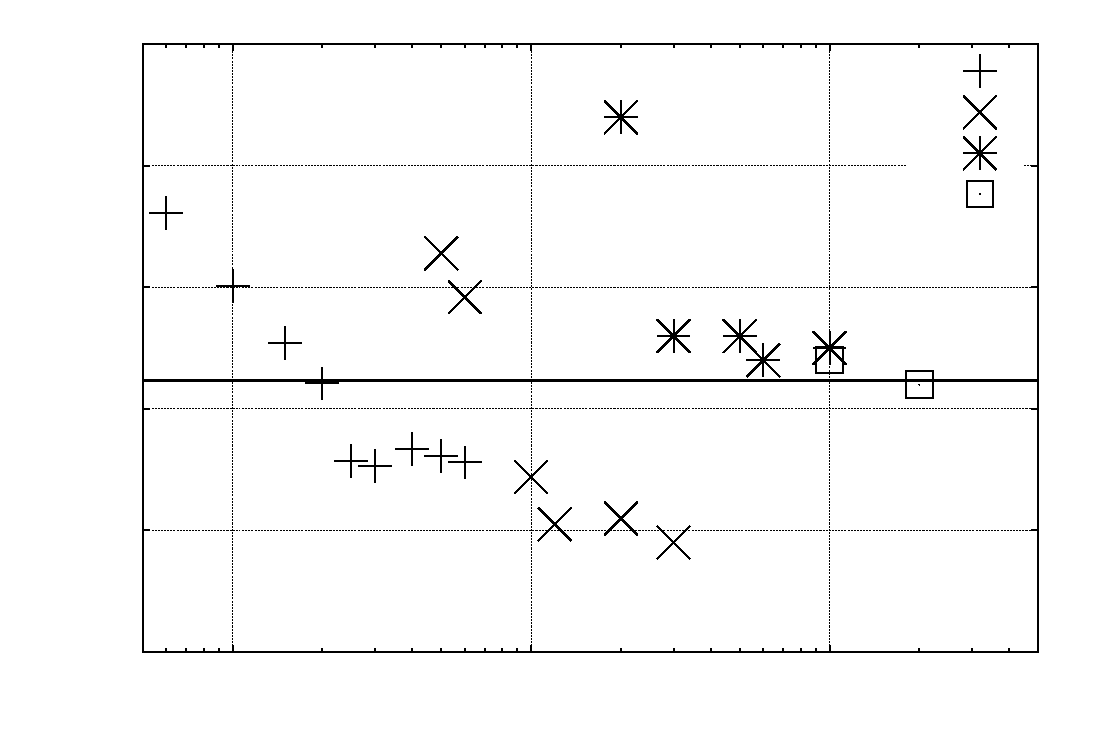
\includegraphics{glycerin}}%
    \gplfronttext
  \end{picture}%
\endgroup

\caption{Dynamická viskozita glycerinu měřená rotačním viskozimetrem s různými rotory (logaritmické měřítko na vodorovné ose)}
\label{grp::rotglyc}
\end{graph}

U škroby je naopak závislost na rychlosti otáčení zřejmá, škrob je tedy nenewtonovská kapalina.
Naměřené hodnoty jsou uvedeny v tabulce \ref{tab::skrob} a zaneseny do grafu \ref{grp::rotskrob}.
Závislost fitujeme funkcí $\eta(F)=A \cdot F^{n-1}$, kde $F$ je frekvence otáčení rotoru v otáčkách za minutu.
Po dosazení $D = 2 \cdot 2\pi \cdot F/60$ dostáváme konstanty v \eqref{eq::fitnenewton}
\begin{equation}
m=\SI{4900(400)}{\milli\Pa\s\tothe{n}} \qquad n = \num{0.42(3)}
\end{equation}

Zdánlivá viskozita se zvyšující se rychlostí klesá $(n < 1)$, škrob je tedy pseudoplastická látka \cite{skripta}.


\begin{tabulka}[htbp]
\centering
\begin{tabular}{ccc|ccc}
rotor & frekvence (\si{\per\minute}) & viskozita (\si{\milli\pascal\s}) & rotor & frekvence (\si{\per\minute}) & viskozita (\si{\milli\pascal\s}) \\
\hline 
\multirow{7}{*}{L2} & 10 & 3000 & \multirow{2}{*}{L2} & 5 & 4888 \\
& 12 & 2670 & & 6 & 4405 \\
& 20 & 1980 & & & \\
& 30 & 1910 & & & \\
& 50 & 1310 & & & \\
& 60 & 1200 & & & \\
& 100 & 950 & & & \\
\end{tabular}
\caption{Naměřené zdánlivé viskozity škrobu rotačním viskozimetrem}
\label{tab::skrob}
\end{tabulka}


\begin{graph}[htbp] 
\centering
% GNUPLOT: LaTeX picture with Postscript
\begingroup
  \makeatletter
  \providecommand\color[2][]{%
    \GenericError{(gnuplot) \space\space\space\@spaces}{%
      Package color not loaded in conjunction with
      terminal option `colourtext'%
    }{See the gnuplot documentation for explanation.%
    }{Either use 'blacktext' in gnuplot or load the package
      color.sty in LaTeX.}%
    \renewcommand\color[2][]{}%
  }%
  \providecommand\includegraphics[2][]{%
    \GenericError{(gnuplot) \space\space\space\@spaces}{%
      Package graphicx or graphics not loaded%
    }{See the gnuplot documentation for explanation.%
    }{The gnuplot epslatex terminal needs graphicx.sty or graphics.sty.}%
    \renewcommand\includegraphics[2][]{}%
  }%
  \providecommand\rotatebox[2]{#2}%
  \@ifundefined{ifGPcolor}{%
    \newif\ifGPcolor
    \GPcolorfalse
  }{}%
  \@ifundefined{ifGPblacktext}{%
    \newif\ifGPblacktext
    \GPblacktexttrue
  }{}%
  % define a \g@addto@macro without @ in the name:
  \let\gplgaddtomacro\g@addto@macro
  % define empty templates for all commands taking text:
  \gdef\gplbacktext{}%
  \gdef\gplfronttext{}%
  \makeatother
  \ifGPblacktext
    % no textcolor at all
    \def\colorrgb#1{}%
    \def\colorgray#1{}%
  \else
    % gray or color?
    \ifGPcolor
      \def\colorrgb#1{\color[rgb]{#1}}%
      \def\colorgray#1{\color[gray]{#1}}%
      \expandafter\def\csname LTw\endcsname{\color{white}}%
      \expandafter\def\csname LTb\endcsname{\color{black}}%
      \expandafter\def\csname LTa\endcsname{\color{black}}%
      \expandafter\def\csname LT0\endcsname{\color[rgb]{1,0,0}}%
      \expandafter\def\csname LT1\endcsname{\color[rgb]{0,1,0}}%
      \expandafter\def\csname LT2\endcsname{\color[rgb]{0,0,1}}%
      \expandafter\def\csname LT3\endcsname{\color[rgb]{1,0,1}}%
      \expandafter\def\csname LT4\endcsname{\color[rgb]{0,1,1}}%
      \expandafter\def\csname LT5\endcsname{\color[rgb]{1,1,0}}%
      \expandafter\def\csname LT6\endcsname{\color[rgb]{0,0,0}}%
      \expandafter\def\csname LT7\endcsname{\color[rgb]{1,0.3,0}}%
      \expandafter\def\csname LT8\endcsname{\color[rgb]{0.5,0.5,0.5}}%
    \else
      % gray
      \def\colorrgb#1{\color{black}}%
      \def\colorgray#1{\color[gray]{#1}}%
      \expandafter\def\csname LTw\endcsname{\color{white}}%
      \expandafter\def\csname LTb\endcsname{\color{black}}%
      \expandafter\def\csname LTa\endcsname{\color{black}}%
      \expandafter\def\csname LT0\endcsname{\color{black}}%
      \expandafter\def\csname LT1\endcsname{\color{black}}%
      \expandafter\def\csname LT2\endcsname{\color{black}}%
      \expandafter\def\csname LT3\endcsname{\color{black}}%
      \expandafter\def\csname LT4\endcsname{\color{black}}%
      \expandafter\def\csname LT5\endcsname{\color{black}}%
      \expandafter\def\csname LT6\endcsname{\color{black}}%
      \expandafter\def\csname LT7\endcsname{\color{black}}%
      \expandafter\def\csname LT8\endcsname{\color{black}}%
    \fi
  \fi
  \setlength{\unitlength}{0.0500bp}%
  \begin{picture}(10204.00,6802.00)%
    \gplgaddtomacro\gplbacktext{%
      \csname LTb\endcsname%
      \put(1210,2054){\makebox(0,0)[r]{\strut{} 1000}}%
      \csname LTb\endcsname%
      \put(1210,6537){\makebox(0,0)[r]{\strut{} 10000}}%
      \csname LTb\endcsname%
      \put(4300,484){\makebox(0,0){\strut{} 10}}%
      \csname LTb\endcsname%
      \put(8533,484){\makebox(0,0){\strut{} 100}}%
      \put(176,3620){\rotatebox{-270}{\makebox(0,0){\strut{}Dynamická viskozita (\si{\milli\Pa\s})}}}%
      \put(5574,154){\makebox(0,0){\strut{}Frekvence otáčení (\si{\per\minute})}}%
    }%
    \gplgaddtomacro\gplfronttext{%
      \csname LTb\endcsname%
      \put(8820,6278){\makebox(0,0)[r]{\strut{}L2}}%
      \csname LTb\endcsname%
      \put(8820,5885){\makebox(0,0)[r]{\strut{}L3}}%
    }%
    \gplbacktext
    \put(0,0){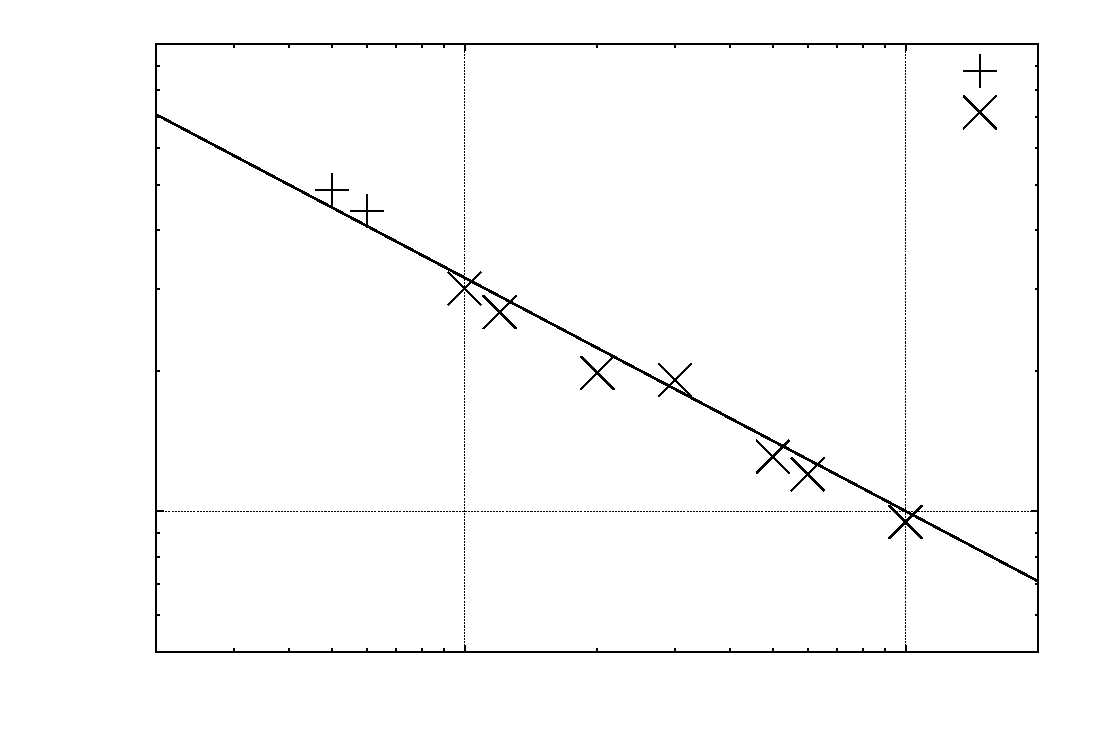
\includegraphics{skrob}}%
    \gplfronttext
  \end{picture}%
\endgroup

\caption{Zdánlivá viskozita škrobu v závislosti na rychlosti otáčení (logaritmické měřítko u obou os)}
\label{grp::rotskrob}
\end{graph}

Kuličkový viskozimetr byl naplněn bezvodým glycerinem (\SI{99.5}{\percent}), jeho hustotu udává \cite{skripta} při naší teplotě \SI{1.257(1)}{\g\per\cm\cubed}.
Naměřené hodnoty jsou uvedeny v tabulce \ref{tab::teplota} a zaneseny do grafů \ref{grp::kulickovej} a \ref{grp::kulickovejadapt}.
Ze směrnice přímky \eqref{eq::primka} určíme aktivační energii $\epsilon_A = $(\num{1.00(2)})\,\SI{e10}{\joule}.

\begin{tabulka}[htbp]
\centering
\begin{tabular}{ccc}
teplota (\si{\degreeCelsius}) & čas (\si{\s}) & viskozita (\si{\milli\pascal\s}) \\ \hline 
25.2	&		183	& 888 \\
26.2	&		173	& 839 \\
27.1	&		160	& 776 \\
28.2	&		146	& 708 \\
29.1	&		135	& 655 \\
30.1	&		124	& 602 \\
31.1	&		115	& 558 \\
32.1	&		107	& 519 \\
33		&		99	& 480 \\
34		&		92	& 446 \\
35		&		86	& 417 \\
\end{tabular}
\caption{Naměřené hodnoty kuličkovým viskozimetrem}
\label{tab::teplota}
\end{tabulka}


\begin{graph}[htbp] 
\centering
% GNUPLOT: LaTeX picture with Postscript
\begingroup
  \makeatletter
  \providecommand\color[2][]{%
    \GenericError{(gnuplot) \space\space\space\@spaces}{%
      Package color not loaded in conjunction with
      terminal option `colourtext'%
    }{See the gnuplot documentation for explanation.%
    }{Either use 'blacktext' in gnuplot or load the package
      color.sty in LaTeX.}%
    \renewcommand\color[2][]{}%
  }%
  \providecommand\includegraphics[2][]{%
    \GenericError{(gnuplot) \space\space\space\@spaces}{%
      Package graphicx or graphics not loaded%
    }{See the gnuplot documentation for explanation.%
    }{The gnuplot epslatex terminal needs graphicx.sty or graphics.sty.}%
    \renewcommand\includegraphics[2][]{}%
  }%
  \providecommand\rotatebox[2]{#2}%
  \@ifundefined{ifGPcolor}{%
    \newif\ifGPcolor
    \GPcolorfalse
  }{}%
  \@ifundefined{ifGPblacktext}{%
    \newif\ifGPblacktext
    \GPblacktexttrue
  }{}%
  % define a \g@addto@macro without @ in the name:
  \let\gplgaddtomacro\g@addto@macro
  % define empty templates for all commands taking text:
  \gdef\gplbacktext{}%
  \gdef\gplfronttext{}%
  \makeatother
  \ifGPblacktext
    % no textcolor at all
    \def\colorrgb#1{}%
    \def\colorgray#1{}%
  \else
    % gray or color?
    \ifGPcolor
      \def\colorrgb#1{\color[rgb]{#1}}%
      \def\colorgray#1{\color[gray]{#1}}%
      \expandafter\def\csname LTw\endcsname{\color{white}}%
      \expandafter\def\csname LTb\endcsname{\color{black}}%
      \expandafter\def\csname LTa\endcsname{\color{black}}%
      \expandafter\def\csname LT0\endcsname{\color[rgb]{1,0,0}}%
      \expandafter\def\csname LT1\endcsname{\color[rgb]{0,1,0}}%
      \expandafter\def\csname LT2\endcsname{\color[rgb]{0,0,1}}%
      \expandafter\def\csname LT3\endcsname{\color[rgb]{1,0,1}}%
      \expandafter\def\csname LT4\endcsname{\color[rgb]{0,1,1}}%
      \expandafter\def\csname LT5\endcsname{\color[rgb]{1,1,0}}%
      \expandafter\def\csname LT6\endcsname{\color[rgb]{0,0,0}}%
      \expandafter\def\csname LT7\endcsname{\color[rgb]{1,0.3,0}}%
      \expandafter\def\csname LT8\endcsname{\color[rgb]{0.5,0.5,0.5}}%
    \else
      % gray
      \def\colorrgb#1{\color{black}}%
      \def\colorgray#1{\color[gray]{#1}}%
      \expandafter\def\csname LTw\endcsname{\color{white}}%
      \expandafter\def\csname LTb\endcsname{\color{black}}%
      \expandafter\def\csname LTa\endcsname{\color{black}}%
      \expandafter\def\csname LT0\endcsname{\color{black}}%
      \expandafter\def\csname LT1\endcsname{\color{black}}%
      \expandafter\def\csname LT2\endcsname{\color{black}}%
      \expandafter\def\csname LT3\endcsname{\color{black}}%
      \expandafter\def\csname LT4\endcsname{\color{black}}%
      \expandafter\def\csname LT5\endcsname{\color{black}}%
      \expandafter\def\csname LT6\endcsname{\color{black}}%
      \expandafter\def\csname LT7\endcsname{\color{black}}%
      \expandafter\def\csname LT8\endcsname{\color{black}}%
    \fi
  \fi
  \setlength{\unitlength}{0.0500bp}%
  \begin{picture}(10204.00,6802.00)%
    \gplgaddtomacro\gplbacktext{%
      \csname LTb\endcsname%
      \put(1078,704){\makebox(0,0)[r]{\strut{} 300}}%
      \csname LTb\endcsname%
      \put(1078,1537){\makebox(0,0)[r]{\strut{} 400}}%
      \csname LTb\endcsname%
      \put(1078,2371){\makebox(0,0)[r]{\strut{} 500}}%
      \csname LTb\endcsname%
      \put(1078,3204){\makebox(0,0)[r]{\strut{} 600}}%
      \csname LTb\endcsname%
      \put(1078,4037){\makebox(0,0)[r]{\strut{} 700}}%
      \csname LTb\endcsname%
      \put(1078,4870){\makebox(0,0)[r]{\strut{} 800}}%
      \csname LTb\endcsname%
      \put(1078,5704){\makebox(0,0)[r]{\strut{} 900}}%
      \csname LTb\endcsname%
      \put(1078,6537){\makebox(0,0)[r]{\strut{} 1000}}%
      \csname LTb\endcsname%
      \put(1210,484){\makebox(0,0){\strut{} 24}}%
      \csname LTb\endcsname%
      \put(2643,484){\makebox(0,0){\strut{} 26}}%
      \csname LTb\endcsname%
      \put(4076,484){\makebox(0,0){\strut{} 28}}%
      \csname LTb\endcsname%
      \put(5509,484){\makebox(0,0){\strut{} 30}}%
      \csname LTb\endcsname%
      \put(6941,484){\makebox(0,0){\strut{} 32}}%
      \csname LTb\endcsname%
      \put(8374,484){\makebox(0,0){\strut{} 34}}%
      \csname LTb\endcsname%
      \put(9807,484){\makebox(0,0){\strut{} 36}}%
      \put(176,3620){\rotatebox{-270}{\makebox(0,0){\strut{}Dynamická viskozita (\si{\milli\Pa\s})}}}%
      \put(5508,154){\makebox(0,0){\strut{}Teplota (\si{\degreeCelsius})}}%
    }%
    \gplgaddtomacro\gplfronttext{%
    }%
    \gplbacktext
    \put(0,0){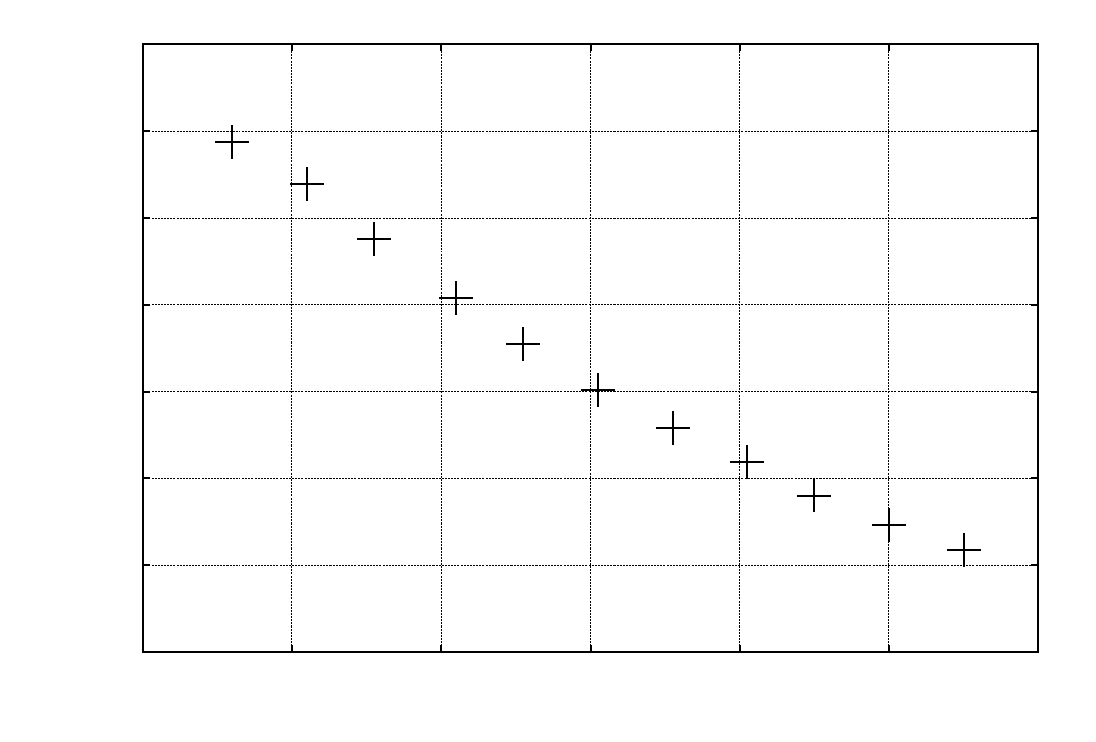
\includegraphics{kulickovej}}%
    \gplfronttext
  \end{picture}%
\endgroup

\caption{Závislost viskozity glycerinu na teplotě, měřeno kuličkovým viskozimetrem}
\label{grp::kulickovej}
\end{graph}

\begin{graph}[htbp] 
\centering
% GNUPLOT: LaTeX picture with Postscript
\begingroup
  \makeatletter
  \providecommand\color[2][]{%
    \GenericError{(gnuplot) \space\space\space\@spaces}{%
      Package color not loaded in conjunction with
      terminal option `colourtext'%
    }{See the gnuplot documentation for explanation.%
    }{Either use 'blacktext' in gnuplot or load the package
      color.sty in LaTeX.}%
    \renewcommand\color[2][]{}%
  }%
  \providecommand\includegraphics[2][]{%
    \GenericError{(gnuplot) \space\space\space\@spaces}{%
      Package graphicx or graphics not loaded%
    }{See the gnuplot documentation for explanation.%
    }{The gnuplot epslatex terminal needs graphicx.sty or graphics.sty.}%
    \renewcommand\includegraphics[2][]{}%
  }%
  \providecommand\rotatebox[2]{#2}%
  \@ifundefined{ifGPcolor}{%
    \newif\ifGPcolor
    \GPcolorfalse
  }{}%
  \@ifundefined{ifGPblacktext}{%
    \newif\ifGPblacktext
    \GPblacktexttrue
  }{}%
  % define a \g@addto@macro without @ in the name:
  \let\gplgaddtomacro\g@addto@macro
  % define empty templates for all commands taking text:
  \gdef\gplbacktext{}%
  \gdef\gplfronttext{}%
  \makeatother
  \ifGPblacktext
    % no textcolor at all
    \def\colorrgb#1{}%
    \def\colorgray#1{}%
  \else
    % gray or color?
    \ifGPcolor
      \def\colorrgb#1{\color[rgb]{#1}}%
      \def\colorgray#1{\color[gray]{#1}}%
      \expandafter\def\csname LTw\endcsname{\color{white}}%
      \expandafter\def\csname LTb\endcsname{\color{black}}%
      \expandafter\def\csname LTa\endcsname{\color{black}}%
      \expandafter\def\csname LT0\endcsname{\color[rgb]{1,0,0}}%
      \expandafter\def\csname LT1\endcsname{\color[rgb]{0,1,0}}%
      \expandafter\def\csname LT2\endcsname{\color[rgb]{0,0,1}}%
      \expandafter\def\csname LT3\endcsname{\color[rgb]{1,0,1}}%
      \expandafter\def\csname LT4\endcsname{\color[rgb]{0,1,1}}%
      \expandafter\def\csname LT5\endcsname{\color[rgb]{1,1,0}}%
      \expandafter\def\csname LT6\endcsname{\color[rgb]{0,0,0}}%
      \expandafter\def\csname LT7\endcsname{\color[rgb]{1,0.3,0}}%
      \expandafter\def\csname LT8\endcsname{\color[rgb]{0.5,0.5,0.5}}%
    \else
      % gray
      \def\colorrgb#1{\color{black}}%
      \def\colorgray#1{\color[gray]{#1}}%
      \expandafter\def\csname LTw\endcsname{\color{white}}%
      \expandafter\def\csname LTb\endcsname{\color{black}}%
      \expandafter\def\csname LTa\endcsname{\color{black}}%
      \expandafter\def\csname LT0\endcsname{\color{black}}%
      \expandafter\def\csname LT1\endcsname{\color{black}}%
      \expandafter\def\csname LT2\endcsname{\color{black}}%
      \expandafter\def\csname LT3\endcsname{\color{black}}%
      \expandafter\def\csname LT4\endcsname{\color{black}}%
      \expandafter\def\csname LT5\endcsname{\color{black}}%
      \expandafter\def\csname LT6\endcsname{\color{black}}%
      \expandafter\def\csname LT7\endcsname{\color{black}}%
      \expandafter\def\csname LT8\endcsname{\color{black}}%
    \fi
  \fi
  \setlength{\unitlength}{0.0500bp}%
  \begin{picture}(10204.00,6802.00)%
    \gplgaddtomacro\gplbacktext{%
      \csname LTb\endcsname%
      \put(946,1028){\makebox(0,0)[r]{\strut{} 6}}%
      \csname LTb\endcsname%
      \put(946,2324){\makebox(0,0)[r]{\strut{} 6.2}}%
      \csname LTb\endcsname%
      \put(946,3621){\makebox(0,0)[r]{\strut{} 6.4}}%
      \csname LTb\endcsname%
      \put(946,4917){\makebox(0,0)[r]{\strut{} 6.6}}%
      \csname LTb\endcsname%
      \put(946,6213){\makebox(0,0)[r]{\strut{} 6.8}}%
      \csname LTb\endcsname%
      \put(1078,484){\makebox(0,0){\strut{} 0.00324}}%
      \csname LTb\endcsname%
      \put(2533,484){\makebox(0,0){\strut{} 0.00326}}%
      \csname LTb\endcsname%
      \put(3988,484){\makebox(0,0){\strut{} 0.00328}}%
      \csname LTb\endcsname%
      \put(5443,484){\makebox(0,0){\strut{} 0.0033}}%
      \csname LTb\endcsname%
      \put(6897,484){\makebox(0,0){\strut{} 0.00332}}%
      \csname LTb\endcsname%
      \put(8352,484){\makebox(0,0){\strut{} 0.00334}}%
      \csname LTb\endcsname%
      \put(9807,484){\makebox(0,0){\strut{} 0.00336}}%
      \put(176,3620){\rotatebox{-270}{\makebox(0,0){\strut{}$\ln(\frac{\eta}{\SI{1}{\milli\pascal\s}}$)}}}%
      \put(5442,154){\makebox(0,0){\strut{}$\frac{1}{T}$ (\si{\per\kelvin})}}%
    }%
    \gplgaddtomacro\gplfronttext{%
    }%
    \gplbacktext
    \put(0,0){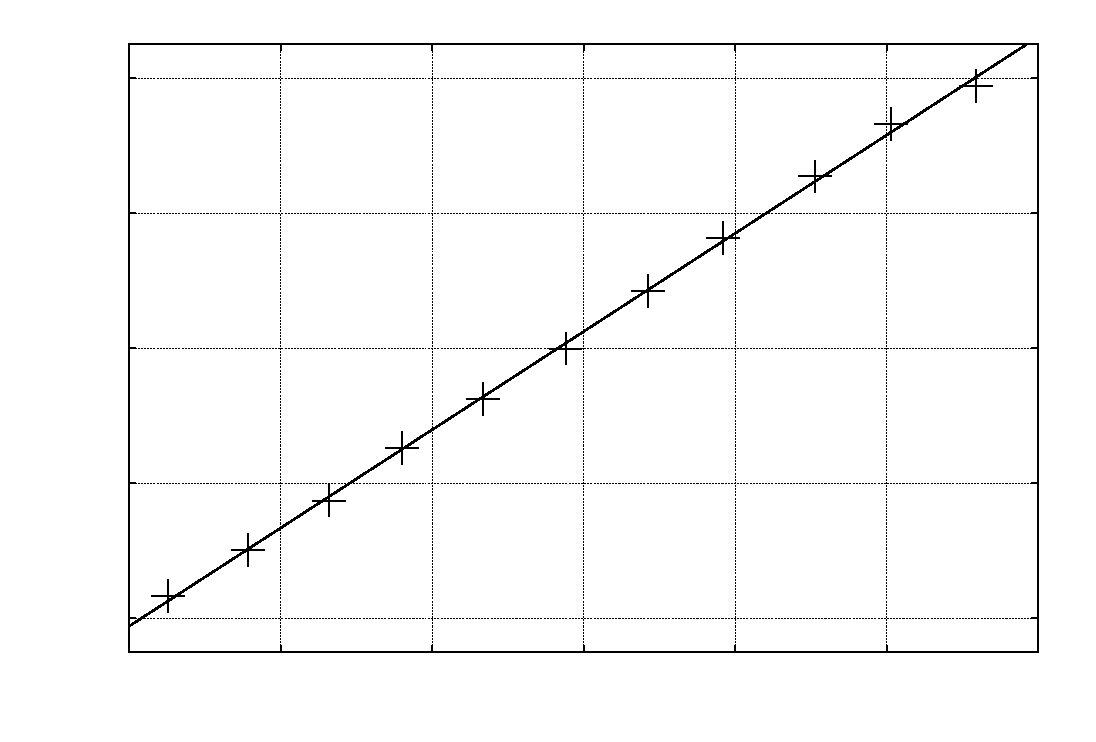
\includegraphics{kulickovejadapt}}%
    \gplfronttext
  \end{picture}%
\endgroup

\caption{Závislost viskozity glycerinu na teplotě (přizpůsobené osy)}
\label{grp::kulickovejadapt}
\end{graph}

Pyknometrickou metodou jsme změřili hustotu glycerinu, který jsme používali v rotačním viskozimetru.
Hmotnost prázdného pyknometru $m_1 = $\SI{24.805(5)}{\g}.
Hmotnost pyknometru naplněného destilovanou vodou $m_2 =$\SI{49.678(5)}{\g}.
Hmotnost pyknometru naplněného použitým glycerinem $m_3 = $\SI{56.042(5)}{\g}.
Hustota destilované vody při \SI{25.6}{\degreeCelsius} je \SI{997.0(5)}{\g\per\cm\cubed} \cite{hustotavody}.
Hustotu použitého glycerinu jsme podle \eqref{eq::pyknometr} určili jako \SI{1251.8(6)}{\g\per\cm\cubed}.
Podle \cite{skripta} má glycerin tuto hustotu při koncentraci přibližně \SI{97.5}{\percent}.